\documentclass[../../main/thesis_msc.tex]{subfiles}



\begin{document}

    \chapter{Introduction}
    
		The cycle of life and death of stars  baffled astronomers for many years. The study of stellar structure and evolution continues -up to this date- to be of paramount importance, since it is crucial to our understanding of various branches of astronomy, e.g. the structure of galaxies, and chemical history of the Universe.
		
		The aim of this thesis is to investigate and get an insight in one of the most debated topics in Stellar Astrophysics; the connection between the progenitor and remnant masses, especially in the case of double neutron star (DNS) binary systems. The existence of those systems was recently confirmed by the detection of gravitational waves emitted during a merging event, accompanied by the detection of a kilonova -the "afterglow"of such an event- as described in the seminal paper of the LIGO/VIRGO collaborations \citep{ligo}.
		
		In this chapter, a synopsis that extends from the formation to the death of Helium stars will be attempted. A detailed coverage of the principles of stellar evolution is beyond the scope of this thesis and a fundamental knowledge is assumed. Moreover, for the interested reader, there are classical textbooks \citep{Kipp_book, Clayton, Prialnik, Eggleton_book} covering almost every aspect in the field of stellar astrophysics. Nevertheless, for the sake of completeness, a small introduction to several fundamental notions, tailored to our needs, will also be carried out in the next few pages. 
		

    
    
    \section{Helium stars}
    	
    	%A brief explanation of what a Helium star is
    	From the large primordial molecular clouds, protostars are being constantly formed via a process called \emph{gravoturbulent cloud fragmentation}. When the accretion of the surrounding material from the protostellar core ceases, the protostar is said to be in the \emph{pre-main sequence} (PMS) phase of its evolution, and continues to contract under the force of gravity until the central temperature becomes sufficiently high for nuclear fusion reactions on Hydrogen to occur. At this point, the star enters the \emph{main sequence} (MS) evolutionary phase as a zero-age main sequence (ZAMS) star where it will spend most of its life.
    	
    	During the MS stage, the star converts Hydrogen to Helium either via the pp-chain reactions, or via the CNO cycles, depending on its initial mass and chemical composition. Slowly but steadily, the Hydrogen in the core is being consumed by the aforementioned nuclear networks, and Helium builds up forming a Helium core. This process continues until the Hydrogen in the stellar core is depleted, resulting to an inert Hydrogen envelope engulfing the newly formed He-core; subsequently, the star exits the MS phase and the nuclear reactions in its interior that provided the necessary pressure support against gravity, effectively stop. Since the star is not in an equilibrium state anymore, it starts to contract until Hydrogen is ignited in a shell around the inert Helium core. At this point, the star enters the so-called \emph{red-giant branch} (RGB) and the Hydrogen-rich envelope, on top of the H-burning shell, inflates rapidly whilst the He-core continues to contract due to the \emph{mirror principle} \citep[see][p.~369]{Kipp_book}.
    	
    	As we will explain in a moment, the Hydrogen envelope can be lost when the star is in the RGB phase, with more than one ways, exposing the He-core of the star. This naked, Hydrogen deficient, He-core is what we refer to as a \emph{Helium star}. We can classify He-stars into two groups: low-mass \emph{hot subdwarfs} (sd) that can be further subdivided into several categories (e.g. sdB, sdO) based on their spectra, and more massive \emph{Wolf-Rayet} (WR) stars that can also be subdivided into several classes (e.g. WN, WC). For a more detailed discussion we refer the reader to the work of \cite{Han2002, Han2003, Heber2009, Chiosi86, langer12}.


			\subsection{Formation of Helium stars}
			
				%A small section explaining how helium stars are being formed
				Helium stars can be formed either in isolation or as part of a binary system. In both scenarios, the physical mechanism that is responsible for the stripping of the Hydrogen envelope is of the utmost importance.
				
				In the former case of a single He-star, the necessary mass loss is being achieved due to strong, radiation-driven, stellar winds. However, the specifics of such a process have not been fully resolved yet, and an enhanced mass loss scheme, e.g. caused by rotational mixing, magnetic fields, or even strong He-flashes should be considered for the progenitor of the He-star \citep{Sweigart, Heber2009}. 
				
				In the case where the He-star progenitor is part of a binary system, the required strong mass loss can be achieved via different channels, depending on how wide the binary system is. These channels include the stable Roche-lobe overflow (RLO) and the Common Envelope (CE) ejection. We will discuss these mass loss mechanisms below.
				It should be mentioned that sdB stars can also originate from the merging of two Helium white dwarfs (He-WD) in a close binary, resulting to an object with enough mass to ignite Helium \citep{Han2002}.
				
				
			
			\subsection{Evolution of single Helium stars}
			
				%A small section explaining the evolution of single helium stars 
				Once the He-star progenitor has been stripped from its Hydrogen envelope during its RGB phase, the compression of the core continues until it reaches the necessary conditions for Helium to ignite at its centre. The ignition of core Helium burning signifies the transition to the Helium main sequence (He-MS) as a He-ZAMS star (see \hyperref[fig:T_rho_plane_ch1]{Fig 1.1}). The last two concepts are defined in a similar way to the (Hydrogen) main sequence and ZAMS respectively.
				
				During the He-MS stage, the star burns its $^4$He supplies via the triple-alpha process producing Carbon ($^{12}$C) and the stable Oxygen isotope $^{16}$O, as a byproduct. When the Helium in the core is depleted, the contraction/expansion process we described above is repeated; the idle metal core that has been formed, consists mainly of Carbon, Oxygen, Neon, and Magnesium and it is surrounded by a He-rich envelope. This whole structure will contract until Helium is ignited in a shell at the bottom of the envelope, followed by the ignition of Carbon in the centre (given that the star is massive enough). The fate of the He-star at this point depends on its mass; if it has not retain enough mass for Carbon ignition, it will gradually cool off and end its life as a Carbon/Oxygen white dwarf (CO WD). On the other hand, if it is massive enough to ignite Carbon, either on or off centre, its fate could be an Oxygen/Neon/Magnesium white dwarf (ONeMg WD), a hybrid white dwarf (CONeMg WD), or even collapse as a supernova.
				
				\begin{figure}[t]
					\centering
					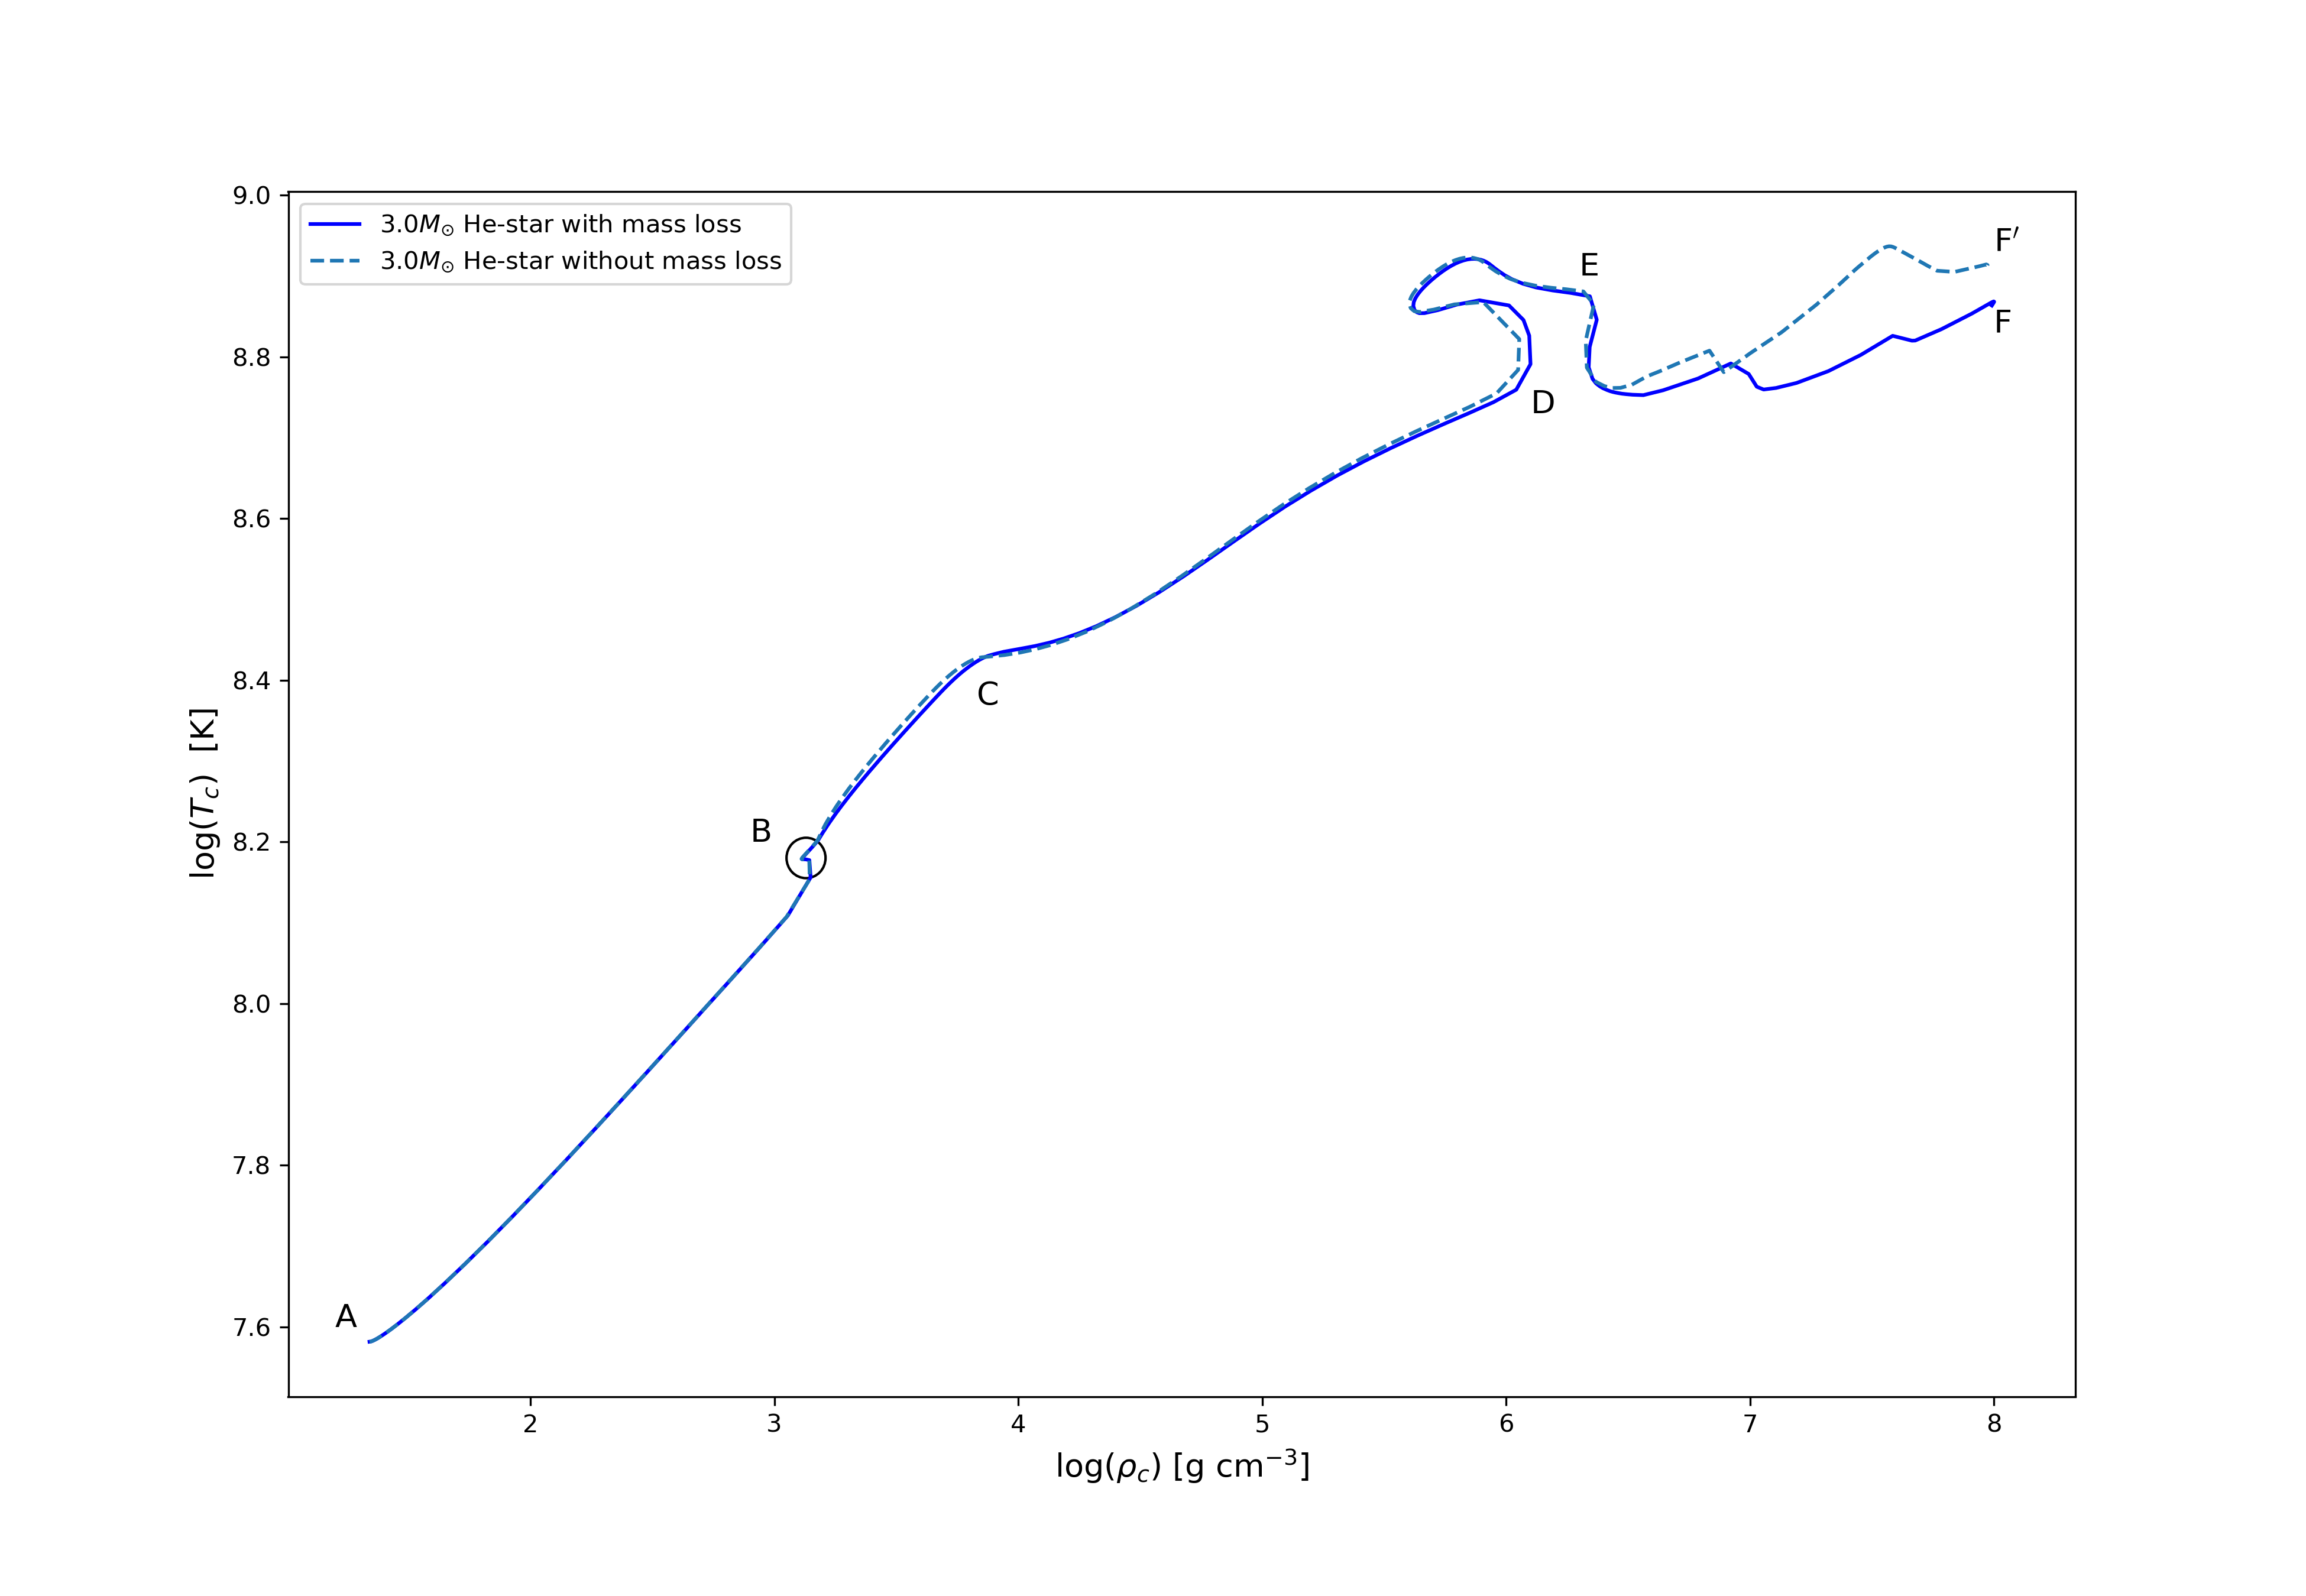
\includegraphics[width=\textwidth]{../figures/chapter1/T_rho_plane_ch1.png}
					\caption{The evolution of a $3.0 M_{\odot}$ He-star, with and without mass loss. The point where the star enters the He-MS as a He-ZAMS can be seen as a small hook inside the black circle. An analytic explanation of the letters along the evolutionary tracks, is provided in the text.}
					\label{fig:T_rho_plane_ch1}
				\end{figure}
				
				To demonstrate the aforementioned stages, the evolutionary track of a $3.0 M_{\odot}$ He-star (with and without mass loss) is illustrated in the $T_c - \rho_c$ plane (\hyperref[fig:T_rho_plane_ch1]{Fig 1.1}) \citep[see also][]{Habets_a, Habets_b, Nomoto1987}. The letters denote the beginning and end of several phases up to the off-centre neon ignition. The A-B phase shows the contraction that follows after the RGB stage of the progenitor. The moment of core He-ignition is denoted by the black circle at point B, and signifies the entrance to the He-MS phase (B-C). At point C, Helium has been exhausted and the core contracts whilst He-shell burning follows. During the D-E phase, the Carbon is ignited in the core making a loop in the diagram around $\rho_c = 10^6$ g cm$^{-3}$. Finally, the E-F/F$^\prime$ shows the Carbon-shell burning along the contraction of the O-Ne-Mg core; at the endpoint (F/F$^\prime$), Neon is ignited off-centre.
				
				For a more complete and comprehensive overview of the evolution of single He-stars, we provide, in the form of a Kippenhahn diagram, the net energy production rate with respect to the internal structure of the $3.0 M_{\odot}$ star (with mass loss) we used in the example above (\hyperref[fig:Kipp_3p0_ch1]{Fig 1.2}). In this diagram, the x-axis expresses the remaining time of the calculations whilst the y-axis shows the inner structure of the star in terms of mass coordinates. The color scale is associated with the energy production.
				
				\begin{figure}[h]
					\centering
					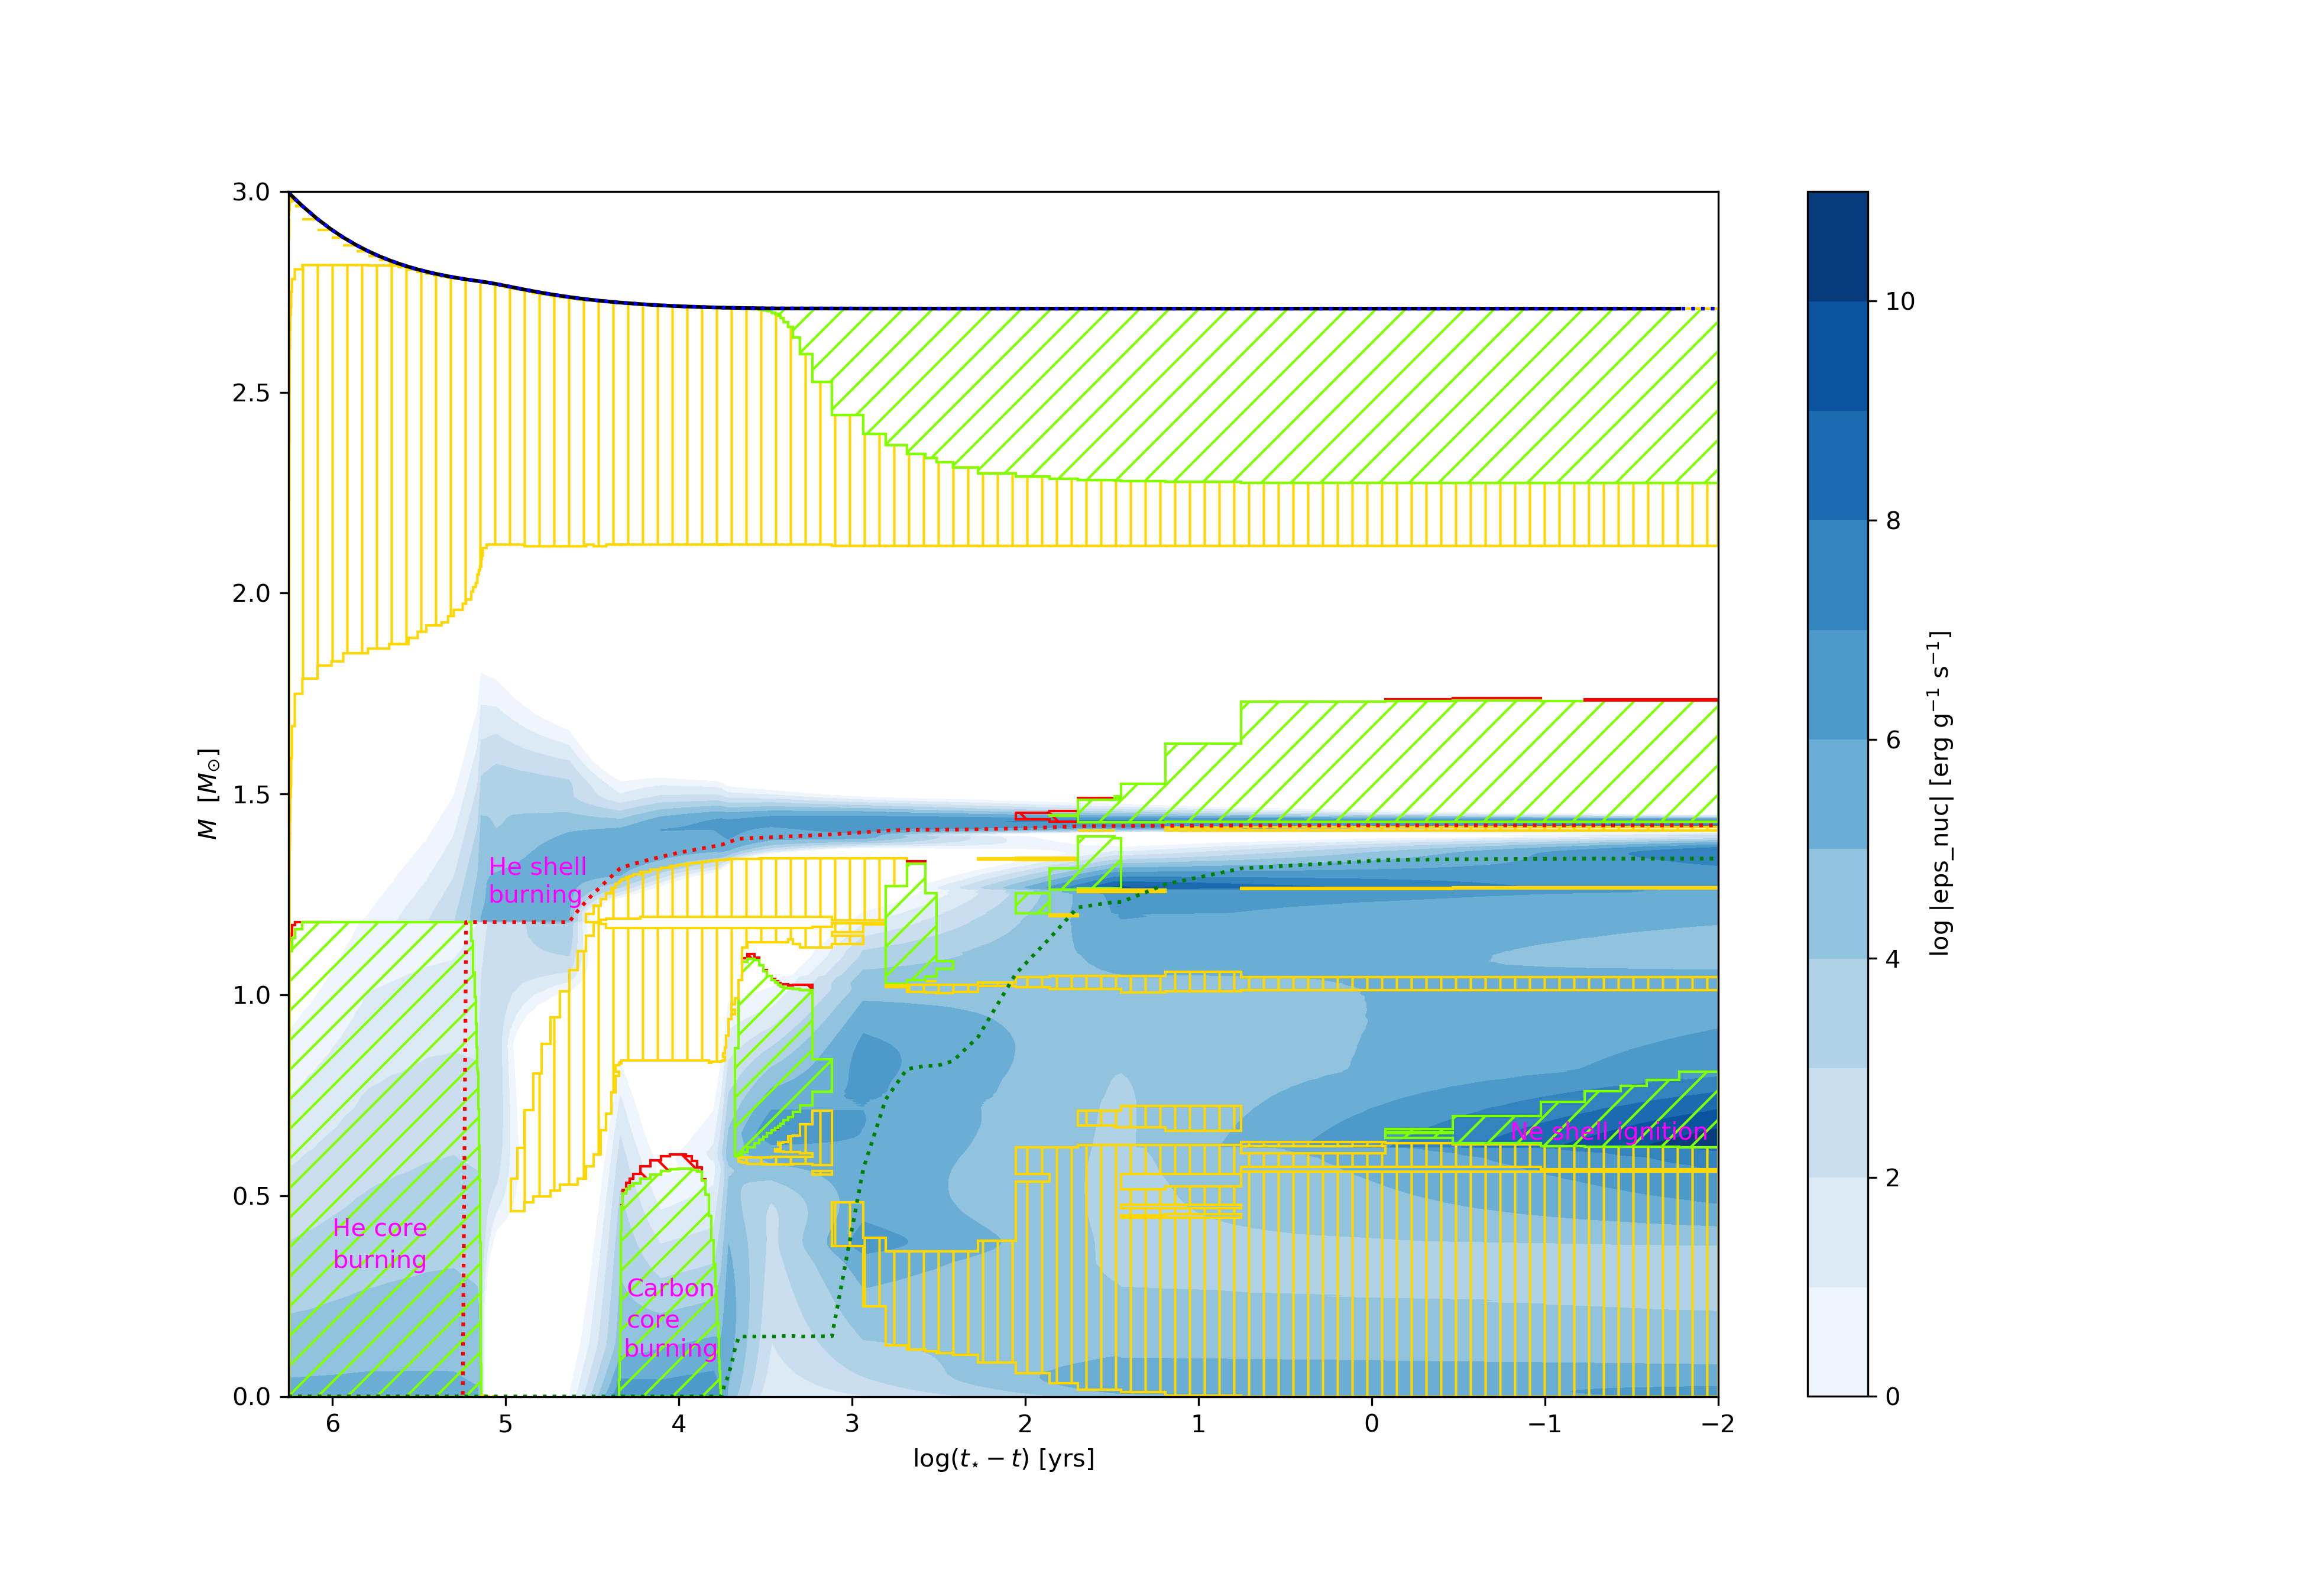
\includegraphics[width=\textwidth]{../figures/chapter1/Kippenhahn_3p0_ch1_with_text_magenta.png}
					\caption{Kippenhahn diagramm for a $3.0 M_{\odot}$ He-star with mass loss. The green and gold hatched areas denote convective and thermohaline mixing respectively. Red solid lines represent areas with semi-convective mixing. The black, red, and green dotted lines show the build-up of Helium, Carbon, and Oxygen core mass respectively}
					\label{fig:Kipp_3p0_ch1}
				\end{figure}
				
				By taking a careful look at \hyperref[fig:Kipp_3p0_ch1]{Fig 1.2}, we observe that during the He-burning in the convective core, the star experiences an approximately $\sim 0.3 M_{\odot}$ mass loss via stellar winds. As a result of this core burning process, a C-core of $\sim 1.2 M_{\odot}$ is formed that continues to grow up to $\sim 1.42 M_{\odot}$ due to He-shell burning. Similarly, an Oxygen core is formed of about $\sim 1.34 M_{\odot}$ as a result of the more advanced burning stages.
				
				
				
				
				
				
					\subsubsection{Mixing mechanisms}
					
						%convection, overshooting, thermohaline
						Although protostars begin their life with, a more or less, uniform elemental composition which is the same as the composition of the cloud they originated from, the ongoing nuclear reactions transform and create new elements that are not necessarily distributed uniformly throughout the stellar interior. This is because there are several ways for a star to stir and mix its material. These mixing mechanisms are usually caused by various instabilities and can contribute on different levels based on specific conditions. In this section we will briefly explain four major mixing processes leaving the effects of rotation for later discussion.
						
						Maybe the most effective way to transfer material is with \emph{convection}. Thermal variations across different shells of the star will lead to density variations and, consequently, to buoyancy driven flows of the fluid. Essentially, what this means is that a hot parcel of fluid will rise due to buoyancy forces and a colder parcel will sink. This process is very efficient for transporting more heavy elements produced in the deep interior of the star towards the surface via bulk motions (dredge-up) and vice versa. The stability of a layer against convection is given by the \emph{Ledoux} criterion
						
						\begin{eqnarray}
							\nabla_{\text{rad}} < \nabla_{\text{ad}} - \frac{\phi}{\delta} \nabla_{\mu}
						\end{eqnarray}
						which, in the case of chemically homogeneous layers ($\nabla_{\mu} = 0$), reduces to the \emph{Schwartzschild} criterion
						
						\begin{eqnarray}
							\nabla_{\text{rad}} < \nabla_{\text{ad}}
						\end{eqnarray}
						For a detailed explanation of the symbols and the implications of those criteria, see \cite[pp.~49-51]{Kipp_book}.
						
						The composition gradient in the Ledoux criterion acts as a stabilizing agent in weakly, thermally unstable regions leading to a slower mixing rate. These zones are not mixed by convection but rather by another process, called \emph{semi-convection} \citep[see][]{Spruit2013, Langer1991}.
						
						Another mechanism that has an important consequence in stellar evolution, is \emph{convective overshooting}. During this phenomenon, a parcel of fluid carried away by convection will overshoot beyond the boundary of the unstable region and into the stable region. This is caused by the inertia of the convective material and thus, it travels some distance further than the region in which it was accelerated until it loses all of its momentum. For this reason, convective overshooting introduces a large uncertainty in the extent of mixed regions.
						
						The fourth major mixing process is called \emph{thermohaline} mixing. It occurs when the molecular weight decreases with depth, e.g. a Helium layer on top of a hydrogen-rich layer due to accretion in a binary system. The heavier elements will eventually sink in whilst the lighter material will rise, re-establishing the mean molecular weight being larger as we move towards the centre of the star. However, thermohaline mixing is believed to play a lesser role in the evolution of single stars and becomes important in accreting binaries \citep[see also][]{Cantiello, Charbonnel}.
		
						
						
						
						
					\subsubsection{Effects of rotation}
					
						%Rotational mixing 
						The evolution of stars can be significantly altered if they are rotating. This is true for most -if not all- stars found in nature, since they inherit angular momentum during the collapse of the already turbulent molecular cloud they originated from. Rotation can influence the shape of stars, their lifetimes since the centrifugal force lowers the internal pressure that is necessary to balance gravity, and their abundance profiles. The latter is a result of several rotation-induced instabilities like the Eddington-Sweet circulation, the dynamical shear instability, and the secular shear instability, to name a few. Especially the Eddington-Sweet circulation and the shear instability play an important role to the transportation of angular momentum between different layers of the star. 
						
						The importance of rotational mixing is difficult to be overstated. As an example, we mention the results of \cite{Maeder1987} who found that, for massive stars, a bifurcation of the evolutionary tracks in the Hertzprung-Russel diagram appears around a critical rotation. This is caused by the inability of the composition gradient ($\nabla_{\mu}$) to prevent turbulent diffusion above this critical rotation, thus the diffusive mixing leads to an almost chemically homogeneous evolution, i.e. the star exhibits the same composition everywhere. These homogeneous models are likely to result to the formation of WR stars before the end of their Hydrogen-burning phase, which increases the WR lifetime, and potentially lead to the formation of gamma-ray bursts in low-metallicity environments \citep{Yoon2005}.
						
						A detailed coverage of the effects of rotation in stellar evolution is offered by \cite{Langer1997, Heger2000, Hirschi, Maeder2006, langer12, Palacios}. More on the rotation-driven transportation of anglular momentum and associated mechanisms can be found in \cite{Heger2005, langer12} as well as in the work of \cite{Spruit2002} where a discussion on the importance of dynamo-generated magnetic fields takes place.
						
						
					\subsubsection{Stellar winds and mass loss}
					
						%Importance of mass loss in the evolution of stellar winds and Wolf-Rayet stars + magnetic braking --> connection to angular momentum losses.
						It has been long since we first discovered that stars experience a continuous outflow of material from their surface causing them to gradually lose a significant fraction of their initial mass. This ejection of material is called \emph{stellar wind} and several mechanisms trying to explain its origin have been proposed over the years.
						
						Stellar winds do not affect all stars in the same way; it depends on the mass of the star and its current evolutionary stage. Low-mass stars that are in the MS phase, like our Sun, are hardly influenced from the generated winds. However, more massive and post-MS stars experience strong, usually radiation accelerated \footnote{These winds can be driven either by radiation pressure on dust condensations that have been formed in the upper atmosphere of stars, or by radiaton pressure on the resonance absorption lines of metals such as carbon and nitrogen.}, winds that peel off large quantities of mass, and changing this way their surface chemical composition. The mass loss rates and the terminal velocities of these winds appear to vary significantly with luminosity, temperature, metallicity, and other global stellar parameters such as the radius \citep{Hamann1982, deJager1988, Nugis2000, yoon17}.
						
						Observations of spectral features have allowed us to establish several empirical relations and constraints for the mass loss rates; especially in the case of WR stars which are known for their strong optically thick winds, the mass loss rates have been revised downwards by almost an order of magnitude \citep{Nugis2000} compared to earlier estimations \citep{Hamann1995, Langer1989} due to the influence of clumping and the asymmetrical structure of the winds. The prescription of \cite{Nugis2000} is currently the most popular for the mass loss rate of WR stars, although \cite{yoon17} raises a word of caution since in the aforementioned prescription, the considered metallicity dependece is not related to the initial metallicity, but rather to the self-enrichment of Carbon and Oxygen at the surface due to mass loss.
						
						Finally, it should be mentioned that in the case of rotating stars, stellar winds will also carry away some of the specific angular momentum of the star along with the ejecta material. Additionally, magnetic fields coupled to the wind plasma in a co-rotation, will slow down the spin of the star which, in turn, will affect the mass loss rate and the angular momentum losses of the system. This is known as \emph{magnetic braking} and plays an important role in stellar evolution, especially in the case of binary systems. For a complete review of our current understanding of stellar winds see \cite{Lamers, smith14}.
						
					
				
	\section{Evolution of binary systems}
	
		%Few words about how most stars form in binary systems, detached, semi-detached and contact binaries
		So far we have concerned ourselves with the evolution of single He-stars. However, the majority of stars are formed in binary systems, being gravitationally bound to each other, and exhibiting a variety of orbital periods that can range from minutes to millions of years. If the two stars are well separated, then the interaction between them should be minimal and both stars will evolve essentially as if they were isolated. Nevertheless, in the case of a close binary, strong interactions might initiate mass transfer from one star to another, altering significantly their structure, how they evolve, and subsequently, their final fate.
		
		In the next few pages, an attempt to briefly explain the basic concepts that govern any interacting binary system will be made. At the end, we will comment on the formation of double neutron star (DNS) binaries which is of particular interest for the aim of this thesis. For a more detailed coverage of the evolution of binary systems we refer to \cite{podsiadlowski_2014, Postnov2014, Eggleton_book, Tauris_2006}.
		
			\subsection{Interaction and orbital parameters}
			
				%Define Lagrangian points, equipotential surfaces, Roche lobe
				In any multiple star system, the gravitational fields of all interacting components influence the motion of the whole system which is governed by the, well known, Newton's laws of motion. This is dubbed as \emph{n-body problem} and is one of the most notoriously difficult problems in physics since it exhibits a chaotic behaviour with no general analytical solution; for this reason, a numerical approach is required.

				In the case of a binary system, the n-body problem is reduced to the \emph{restricted three-body problem} with the effective gravitational potential 
					\begin{eqnarray}
						\label{eq:eff_potential}
						\Phi = -G \left( \frac{M_1}{r_1} + \frac{M_2}{r_2} \right) - \frac{1}{2} \Omega^2 r_3^2
					\end{eqnarray}
					where a full explanation of the symbols is given in \cite[p.~639]{Tauris_2006}. If we require the cumulative forces acting on a test mass, $m$, to vanish
					\begin{eqnarray}
						\label{eq:cum_force}
						\pmb{F}_t = -m \nabla \Phi = 0
					\end{eqnarray}
				then \hyperref[eq:eff_potential]{eq(1.3)} yields five stationary solutions where the gravitational force cancels out the centrifugal force caused by the relative motion of the two stars around each other. The points where \hyperref[eq:cum_force]{eq(1.4)} holds true, are called \emph{Lagrangian points} or \emph{libration points}, \emph{$L_n$, $n=1,2,3,4,5$}. Hence, if a test mass was to be positioned in any of those five equilibrium points, it would maintain its position relative to the two stars. More information on the stability of Lagrangian points, in the sense of what would happen if one applied a small perturbation on a test mass sitting in a libration point, can be found in \cite{Szebehely, Celletti1990, Schwarz2012}.
				
				\begin{figure}[h]
					\centering
					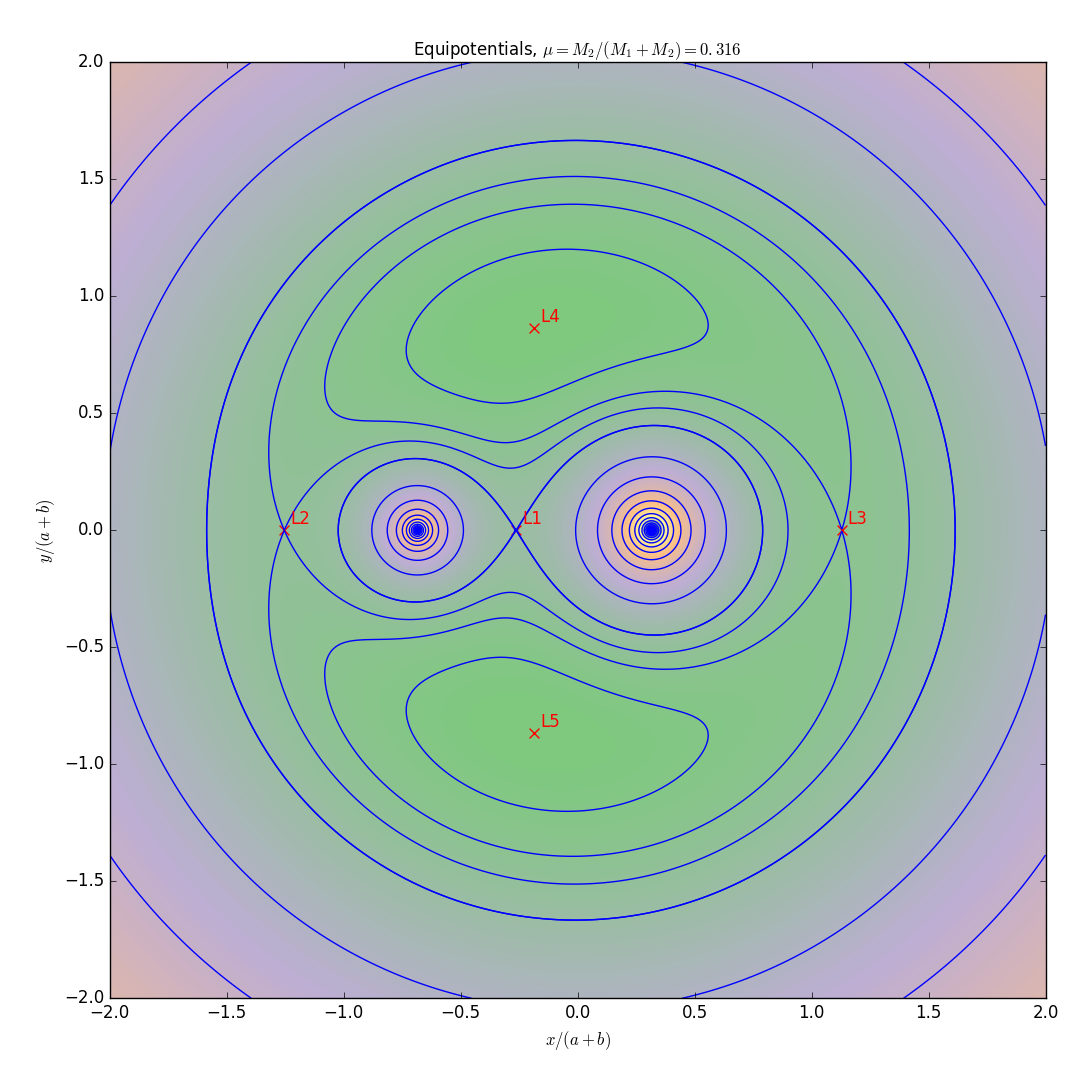
\includegraphics[scale=0.4]{../figures/chapter1/equipotential_surfaces/equipotentials_mu_0_316.png}
					\caption{Equipotential surfaces on the plane of the orbit of a rotating binary with a reduced mass ratio of $\mu = 0.316$. The inner equipotential surface that passes from the $L_1$ Lagrangian point, defines the "teardrop"-shaped Roche-lobes, one for each star. The image was created using a \texttt{python} script, courtesy of \cite{Zingale}.}
					\label{fig:eq_sur}
				\end{figure}
				
				From the five Lagrangian points, the $L_1$ plays a key role in the evolution of binary systems since the equipotential surface \footnote{An equipotential surface is defined as the collection of all points in the system that share the same value of the effective gravitational potential, $\Phi$.} passing through that inner point, defines the \emph{Roche-lobe}. The shape of the equipotential surfaces is illustrated in \hyperref[fig:eq_sur]{Fig 1.3}; they assume a concentric spherical shape in proximity to the two stars whilst, as a result of the combined gravitational influence of the two masses, they get distorded when we move further away.
				
				During the various evolutionary stages, the star might increase its radius to such a degree that the volume of the star exceeds the volume defined by its Roche-lobe. This will cause a transfer of surface material from that star to its companion via the $L_1$ point triggered by the unbalanced pressure in that direction; this process is known as \emph{Roche-lobe overflow} (RLOF) and the donor star can lose a substantial amount of its total mass. Unfortunatelly, there is no analytical expression for the size of a Roche-lobe in a given binary. However, \cite{Eggleton1983} has proposed a numerical approximation of the radius of the Roche-lobe given by \hyperref[eq:rl_radius]{eq(1.5)}
				
				\begin{eqnarray}
					\label{eq:rl_radius}
					R_L = \frac{0.49 q^{2/3}}{0.6 q^{2/3} + \ln(1 + q^{1/3})} \alpha 
				\end{eqnarray}				 
				where $\alpha$ is the orbital separation, and $q \equiv M_{\text{donor}} / M_{\text{accretor}}$ is the mass ratio of the binary components. These are the two most important orbital parameters that we need to know in order to follow the evolution of the binary.
				
				Based on which equipotential surfaces are filled, we can classify binary systems into three categories:
					\begin{enumerate*}[label=(\roman*)]
						\item \emph{detached binaries} where the radii of both stars are much smaller than their orbital separation; neither of the two stars fills its respective Roche-lobe, and they evolve almost independently of each other,
						\item \emph{semi-detached binaries} where only one of the two stars fills its Roche-lobe leading to distortion of the equipotential surfaces from their spherical shape, and mass transfer occurs, and
						\item \emph{contact binaries} where both stars fill their Roche-lobe. This situation results to a shared, common atmosphere that might be ejected, stripping the system from a significant amount of mass.
					\end{enumerate*}									
				

					
			\subsection{Mass transfer}
			
				%Cases A/B/C, (wind mass accretion + Roche lobe overflow) etc			
				
			\subsection{Common envelope}
			
				Explain a little bit in more detail the basics of CE
				
			\subsection{Angular momentum transfer}
			
				Effects of angular momentum transfer + magnetic braking
				
			\subsection{Gravitational waves}
			
				The very basics for GWs and their impact on binary mergers
				
			\subsection{Double neutron star systems}
				
	\section{Stellar transients}
	
		Couple of words for the different types of stellar transients and how can we observe them
		
			\subsection{Classification of Supernovae}
			
				Explain in details the difference between core collapse SNe and type Ia and different subdivision
				
			\subsection{Type Ib/c Supernovae}
			
				Explain in details this particular branch
				
			\subsection{X-ray binaries}
			
				HMXB, LMXB, UCXB
    
    
    \end{document}
    